\section{Budowa pojazdu}
\label{sec:building}
    Inspiracją do stworzenia poniższego projektu były samochody autonomiczne, które najczęściej są pojazdami dwuosiowymi, z jedną osią skrętną i jedną napędową.
    Żadna z nich nie jest ze sobą połączona, co pozwoliło na niezależne sterowanie.
    W konstrukcji zostały użyte dwa silniki prądu stałego, wybrane w rozdziale \ref{sec:engines}, połączone bezpośrednio do tylnych kół.
    \subsection{Przednia oś}
    \label{subsec:drive_axis}
        Układ kierowniczy oparto na serwomechanizmie.
        Na rysunku \ref{fig:frontAxis_model} przedstawiono model tego elementu, zaprojektowanego przez autora.

        \begin{figure}[!ht]
            \centering
            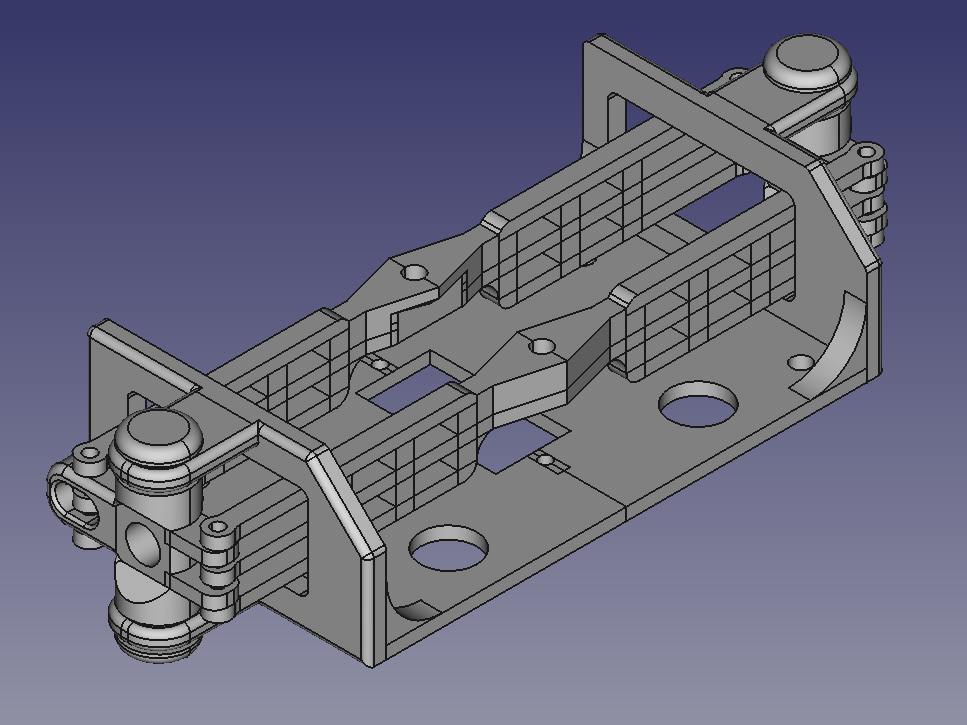
\includegraphics[width=0.7\textwidth]{FronAxis_example.png}
            \caption{Przykładowy układ kierowniczy zaprojektowany w narzędziu FreeCAD}
            \label{fig:frontAxis_model}
        \end{figure}
        Mechanizm ten został rozplanowany w taki sposób, aby środek osi znajdował się w linii ze środkiem serwomechanizmu.
        Dzięki temu ustawiony kąt serwa, odpowiada kątowi skrętu kół.
        Natomiast dużą wadą takiego połączenia jest możliwość jego uszkodzenia, po przekroczeniu maksymalnego zakresu ruchu.

    \subsection{Rama pojazdu}
    Do budowy podwozia została wykorzystana gotowa rama, z poniższego zdjęcia (rys. \ref{fig:test_chassis}), produkowana przez firmę Waveshare.
\clearpage
    \begin{figure}[!ht]
        \centering
        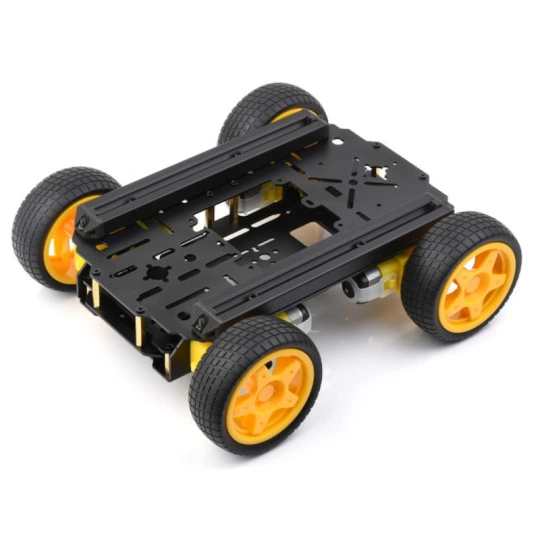
\includegraphics[width=0.7\textwidth]{chassis-waveshare-24419.png}
        \caption{Rama Waveshare 24419}
        Źródło: \href{https://www.waveshare.com/robot-chassis.htm?sku=24419}{waveshare.com}
        \label{fig:test_chassis}
    \end{figure}

    Aby spełnić założenia projektowe, przednia oś konstrukcji została wymieniona na wyżej opisaną (rozdział \ref{subsec:drive_axis}).
    Dodatkowo zmieniono sposób montażu silników, które zamontowano odwrotnie do zaleceń producenta (rys. \ref{fig:motors}), a także zrezygnowano z ,,gumek", odpowiadających za amortyzację.

    \begin{figure}[!ht]
    \centering
    \begin{subfigure}{0.49\textwidth}
        \centering
        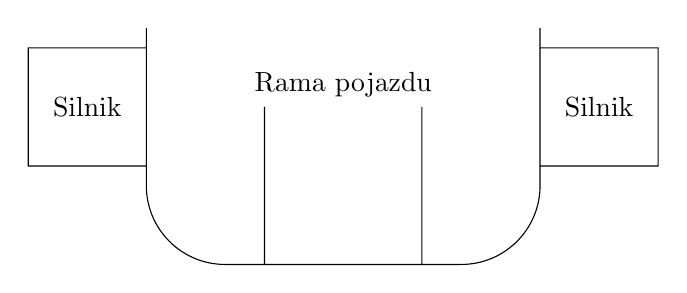
\begin{tikzpicture}
            \draw
                (0, 0) -- ++ (0, -2)
                    arc(0:90:-1)
                    -- ++ (3, 0)
                    arc(-90:0:1)
                    -- ++ (0, 2)

                (0, -0.25) rectangle node[]{Silnik} ++(-1.5, -1.5)
                (5, -0.25) rectangle node[]{Silnik} ++( 1.5, -1.5)


                (1.5, -3) --++(0, 2)
                (3.5, -3) --++(0, 2)
                (2.5, -1) node[above]{Rama pojazdu}
            ;
        \end{tikzpicture}
        \caption{Pierwotne połączenie}
    \end{subfigure}
    \begin{subfigure}{0.49\textwidth}
        \centering
        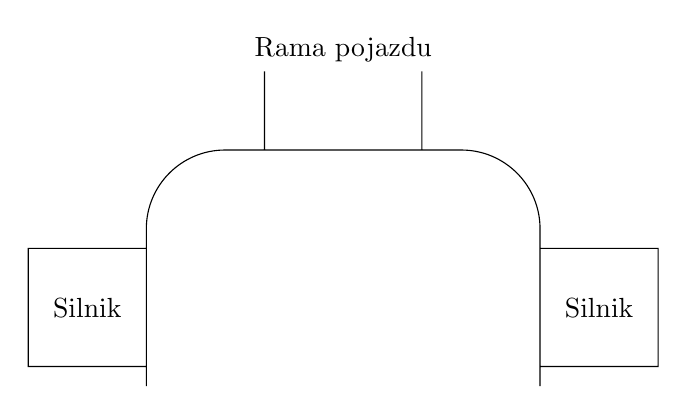
\begin{tikzpicture}
            \draw
                (0, 0) -- ++ (0, 2)
                    arc(0:-90:-1)
                    -- ++ (3, 0)
                    arc(90:0:1)
                    -- ++ (0,-2)

                (0, 0.25) rectangle node[]{Silnik} ++(-1.5, 1.5)
                (5, 0.25) rectangle node[]{Silnik} ++( 1.5, 1.5)

                (1.5, 3) --++(0, 1)
                (3.5, 3) --++(0, 1)
                (2.5, 4) node[above]{Rama pojazdu}
            ;
        \end{tikzpicture}
        \caption{Zastosowane połączenie}
    \end{subfigure}
    \caption{Schemat montażu silników}
    \label{fig:motors}
\end{figure}


    \subsection{Pomiar odległości}
        Współczesne pojazdy autonomiczne wykorzystują układy LIDAR, które pozwalają mierzyć w pełnym zakresie $360^\circ$.
        Jednak w wielu sytuacjach taki pomiar mija się z celem, gdyż znaczna część próbek zostaje odrzucona.
        Same LIDARy zaś są bardzo drogimi urządzeniami, często z niestandardowym sposobem komunikacji (np. za pomocą UART).
        Z tego względu autor zdecydował się na zastosowanie tańszych czujników ToF.
        Trzy takie moduły umieszczono z przodu samochodu, z krokiem co $30^\circ$.
        Na rysunku \ref{fig:ToF_holder} zaprezentowano model mocowania wyżej wymienionych elementów.

        \begin{figure}[!ht]
            \centering
            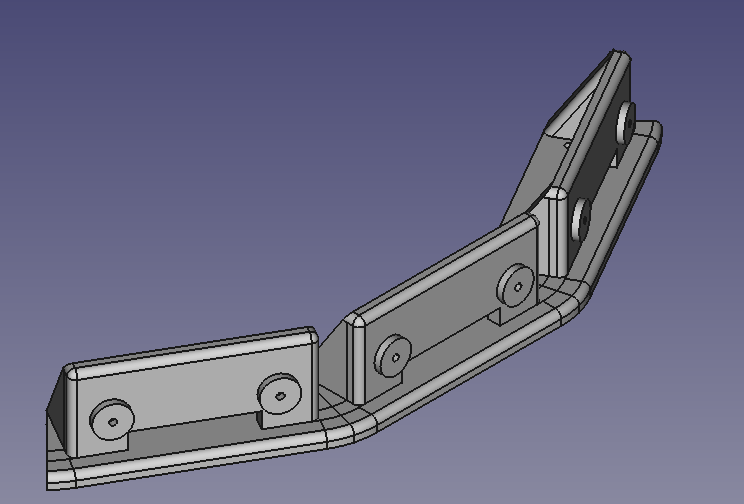
\includegraphics[width=0.7\textwidth]{ToF_holder.png}
            \caption{Mocowanie czujników ToF}
            \label{fig:ToF_holder}
        \end{figure}
